\documentclass[journal]{IEEEtran}
\usepackage{cite}
\usepackage{url}
\usepackage{graphicx}
\usepackage[center]{caption}
\usepackage{listings}
\usepackage{color}
\hyphenation{op-tical net-works semi-conduc-tor}

\linespread{1.2}
\begin{document}
\title{Analysis of an Eulerian Circuit Finding Algorithm}
\author{Anthony~Naddeo}%

% The paper headers
\markboth{Capstone Assignment 1, February 3 2012}%
{Shell \MakeLowercase{\textit{et al.}}: Bare Demo of IEEEtran.cls for Journals}
% The only time the second header will appear is for the odd numbered pages
% after the title page when using the twoside option.

\maketitle

\begin{IEEEkeywords}
Eulerian, algorithm, graph, circuit
\end{IEEEkeywords}





%------------------------------------------------------------
% Section I: Introduction
%------------------------------------------------------------
\section{Introduction} 

\IEEEPARstart{O}{}ur assignment this week asked us to create an algorithm that finds Eulerian circuits in graphs. The purpose of this paper is to prove that the running time of our algorithm is indeed \textit{O(n)} by providing empirical evidence in the form of run times from our implementations. 


%------------------------------------------------------------
% Section I: Results
%------------------------------------------------------------
\section{Results}

In the written section of this assignment I show that the time complexity of this Eulerian circuit finding algorithm is \textit{O(n)}. To provide an empirical proof, I wrote a test program that generates simple Eulerian circuits of any given size \textit{n}, where \textit{n} represents the amount of edges in the graph. The output would be fed to the Java application and the running time recorded with the \texttt{System.currentTimeMillis()} function, taking the average run time from five executions with each \textit{n} tested. The test was split into two timed sections: the amount of time that Jflex and Cup took to parse the input and the amount of time the application took to find the Eulerian circuit from the generated graph. Figure \ref{fig:path} shows the results of the circuit finding algorithm. 

\begin{figure}[h]
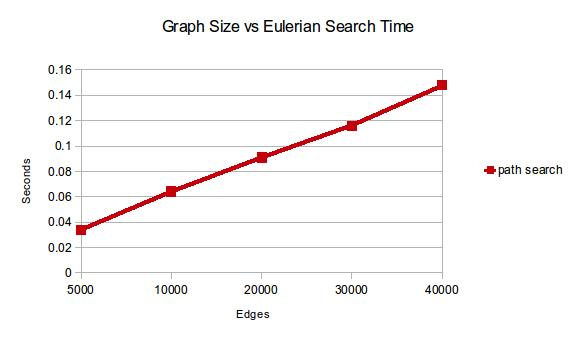
\includegraphics[width=.5\textwidth]{images/path.jpg}
\caption{}
\label{fig:path}
\end{figure}

As previously shown, the time complexity of the algorithm is \textit{O(n)}; it grows linearly as \textit{n} increases. The core of the algorithm consists of a single loop that iterates once for every edge in the graph. The success of this algorithm is contingent upon the data structures holding the graph vertices being sorted in descending order.

\begin{figure}[h]
\begin{lstlisting}[language=java, 
 basicstyle=\footnotesize,  keywordstyle=\textbf]
Vertex current,next;
while(current.degree() > 0){

  next = current.getEdges().get(0);
  Vertex.disconnect(current, next);
  solution.addStep(current.name(), next.name());
  
  current = next;
}
\end{lstlisting}
\caption{Main loop of eulerian circuit algorithm}
\end{figure}

Perhaps of greater interest is the performance of the JFlex and Cup parser. Figure \ref{fig:parse} shows the time that parsing took as \textit{n} increased. The program first parses input and then finds the resulting circuit; each parse time was recorded right before a corresponding circuit finding time.

\begin{figure}[h]
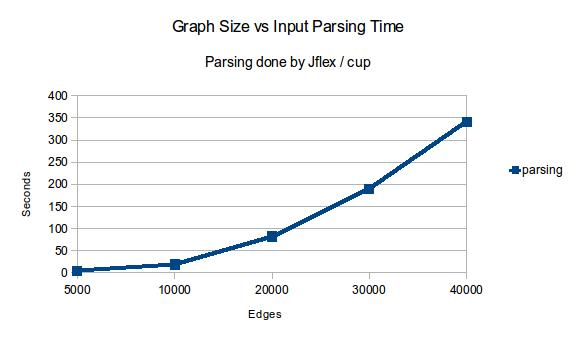
\includegraphics[width=.5\textwidth]{images/parse.jpg}
\caption{}
\label{fig:parse}
\end{figure}

The parser appears to have a polynomial time complexity. Whether this is expected behavior or inefficiency on my part is unknown. 


%------------------------------------------------------------
% Section X: Conclusion
%------------------------------------------------------------
\section{Conclusion}

The results posted in this paper support the previous statement that the algorithm created for this assignment has a time complexity of \textit{O(n)}.




%\appendices
%\begin{thebibliography}{1}
%\bibitem{IEEEhowto:kopka}
%H.~Kopka and P.~W. Daly, \emph{A Guide to \LaTeX}, 3rd~ed.\hskip 1em plus
%  0.5em minus 0.4em\relax Harlow, England: Addison-Wesley, 1999.
%\end{thebibliography}

\end{document}


